\documentclass[12pt, a4paper]{article}

% Preamble

\usepackage[utf8]{inputenc}
\usepackage[english]{babel}
\usepackage[margin=1in]{geometry}
\usepackage[parfill]{parskip}
\usepackage[hidelinks]{hyperref}
\usepackage{graphicx}
\usepackage{listings}
\usepackage{subcaption}
\usepackage{float}
\bibliographystyle{ieeetr}

\title{Summary of the Bachelor thesis ``Decompilation of LLVM IR''}
\date{2014-10-08}

% Document

\begin{document}

\maketitle

This is a summary of a Bachelor thesis written by Simon Moll in 2011, entitled ``Decompilation of LLVM IR''~\cite{decomp_of_llvm}.

Moll's paper explores various techniques for reconstructing high-level primitives from LLVM IR, which is the low-level intermediate representation of the LLVM compiler infrastructure. Or, to phrase it differently; it demonstrates how to turn machine readable code into human readable code, a process known as decompilation.

The LLVM IR language is conceptually a platform-independent RISC assembly language whose control flow is structured using basic blocks. Each basic block consists of a sequence of instructions and ends with a terminator instruction (such as a branch or a function return), which indicates the next basic block to execute. The connections between basic blocks, as specified by the execution flow, may be represented using a Control Flow Graph (CFG), in which each basic block represents a node.

In the following illustrations each letter (A-C) represents a node in a CFG, and each arrow represents the flow of execution from one node to another.

\begin{figure}[H]
   \centering
   \begin{subfigure}[b]{0.2\textwidth}
      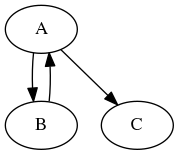
\includegraphics[width=\textwidth]{inc/pre_loop.png}
   \end{subfigure}
   \qquad
   \begin{subfigure}[b]{0.2\textwidth}
      \lstinputlisting{inc/pre_loop.c}
   \end{subfigure}
   \caption{The CFG (left) and pseudo-code (right) of a while-loop.}
\end{figure}

\begin{figure}[H]
   \centering
   \begin{subfigure}[b]{0.15\textwidth}
      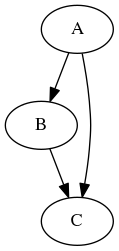
\includegraphics[width=\textwidth]{inc/if.png}
   \end{subfigure}
   \qquad
   \begin{subfigure}[b]{0.2\textwidth}
      \lstinputlisting{inc/if.c}
   \end{subfigure}
   \caption{The CFG (left) and pseudo-code (right) of an if-statement.}
\end{figure}

A key insight provided by the paper is the idea that various high-level primitives, such as while-loops and if-statements, have different patterns in the CFG. This enables the use of pattern matching to reconstruct high-level primitives from lower level representations.

\bibliography{references}

\end{document}
